\documentclass[a4paper, 12pt]{article}

\usepackage[portuges]{babel}
\usepackage[utf8]{inputenc}
\usepackage{amsmath}
\usepackage{indentfirst}
\usepackage{graphicx}
\usepackage{multicol,lipsum}

\begin{document}

\begin{titlepage}
    \begin{center}

        \begin{figure}[!ht]
            \centering
            
\includegraphics[width=10cm]{images/IST.png}
        \end{figure}

        \Huge{Instituto Superior Técnico}\\
        \large{LEEC}\\
        \large{Sinais e Sistemas}\\
        \vspace{15pt}
        \vspace{95pt}
        \textbf{\LARGE{Relatório Laboratório Sinais e Sistemas}}\\
        \vspace{3,5cm}
    \end{center}

    \begin{flushleft}
        \begin{tabbing}
            Aluno: Henrique Machado 103202 \\
            Aluno: Miguel Neves 103462 \\
        \end{tabbing}
    \end{flushleft}
    \vspace{1cm}

    \begin{center}
        \vspace{\fill}
        Janeiro\\
        2023
    \end{center}
\end{titlepage}
%%%%%%%%%%%%%%%%%%%%%%%%%%%%%%%%%%%%%%%%%%%%%%%%%%%%%%%%%%%
% % % % % % % % % % % % % % % % % % % % % % % % % %
\newpage
\tableofcontents
\thispagestyle{empty}
\newpage
\pagenumbering{arabic}
% % % % % % % % % % % % % % % % % % % % % % % % % % %
\section{Sinais Sinusoidais}
\begin{itemize}
    \item \textbf{Q1:} As sinusoidais com frequência mais altas correspondem aos sons mais graves, inversamente, as sinusoidais com frequência mais baixa correspondem aos sons mais graves.
    \item \textbf{Q2:} A frequência minima que nós conseguimos ouvir foi $55hz$ e a frequência máxima que conseguimos ouvir foi $18000hz$.
\end{itemize}
% % % % % % % % % % % % % % % % % % % % % % % % % % %
\vspace{15px}
\section{Notas Musicais}
\begin{itemize}
    \item \textbf{Q3:}
          \begin{enumerate}
              \item[] Mi$_4$: $329.63hz$
              \item[] Fá$_4^\#$: $370.00hz$
              \item[] Sol$_4$: $392.00hz$
              \item[] Si$_4$: $493.89hz$
              \item[] Dó$_5$: $554.37hz$
          \end{enumerate}
\end{itemize}
% % % % % % % % % % % % % % % % % % % % % % % % % % %
\vspace{15px}
\section{Impulso e Degrau Unitários}
\begin{itemize}
    \item \textbf{Q4:} Com base na definição de degrau unitário, $u(at+b)$ pode ser escrito como $u(\pm t - t_0)$ uma vez que: $t_0 = \frac{b}{|a|}$, onde temos que
          \[ \begin{cases}
                  a > 0, & t > 0 \\
                  a < 0, & t < 0
              \end{cases} \]
          Caso $a < 0$, verifica-se uma inversão no tempo do gráfico de $u(t)$.
          \newpage
    \item \textbf{Q5:} $\delta(at) = \frac{1}{\Delta}[u(at) - u(at - \Delta)]$ e $\delta(at) = \underset{{\Delta\to0}}{\lim}\delta_\Delta(at)$, com $a > 0$\vspace{15px}\\
          Para $\delta(t)$\hspace{150px}Para$\delta(at)$\\
          \begin{figure}[!ht]
              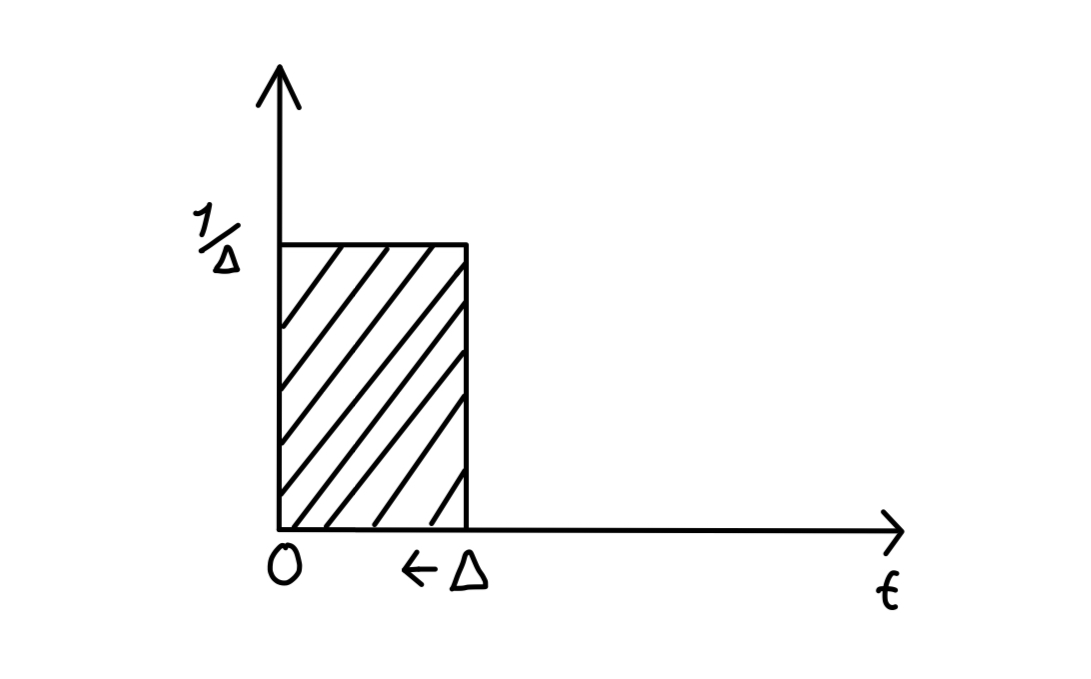
\includegraphics[width=6cm]{images/Graf1.png}
              \hspace{10px}
              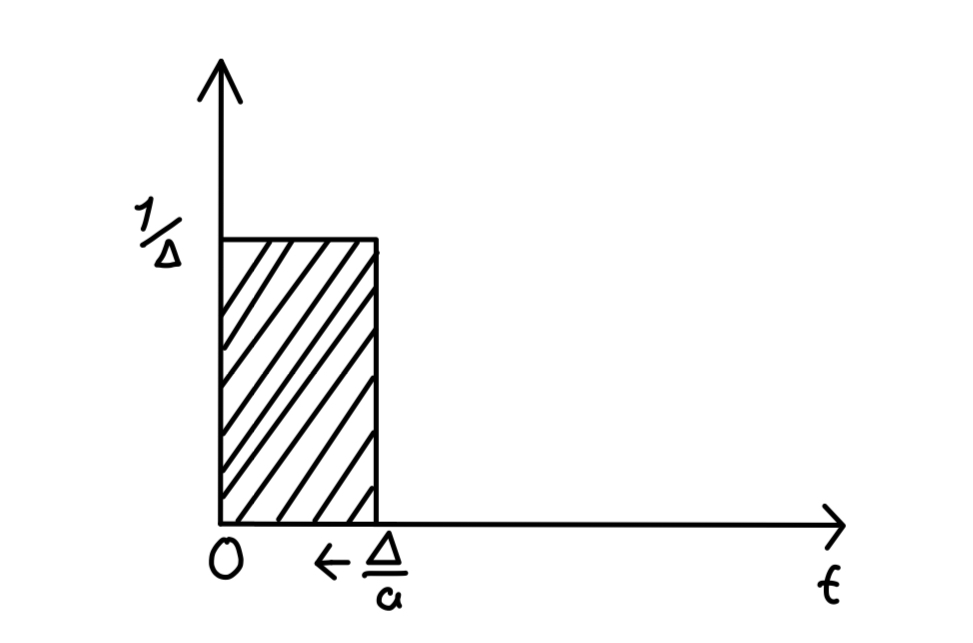
\includegraphics[width=6cm]{images/Graf2.png}
          \end{figure}\\
          Área $ = \frac{1}{\Delta}\times\Delta = 1$\hspace{100px}Área $= \frac{1}{\Delta} \times \frac{\Delta}{a} = \frac{1}{a}$\vspace{15px}\\
          Logo, $\delta(at) = \frac{1}{a}\delta(t)$, com $a > 0$.\vspace{5px}
    \item \textbf{Q6:} Não se verifica nenhuma mudança no gráfico de $\delta(at)$ em relação ao gráfico de $\delta(t)$. No entanto, pelo que foi concluído previamente, o que deveria acontecer seria uma redução da área do impulso devido ao produto pelo termo $\frac{1}{a}$ (sendo $a > 1$) transformação esta que não é visível no visor.
\end{itemize}
\newpage
% % % % % % % % % % % % % % % % % % % % % % % % % % %
\section{Sistemas}
\begin{itemize}
    \item \textbf{Q7:} O sistema apresentado é linear:
          \[x_1(t) \to y_1(t) = x_1(t) + 0.5x_1(t - 0.25)\]
          \[x_2(t) \to y_2(t) = x_2(t) + 0.5x_2(t - 0.25)\]
          $x_3(t) \to$ Combinação linear de $x_1(t)$ e $x_2(t) : x_3(t) = ax_1(t) + bx_2(t)$\vspace{-5px}
          \[y_3(t) = x_3(t) + 0.5x_3(t + 0.25)\]
          \[= ax_1(t) + bx_2(t  ) + 0.5(ax_1(t - 0.25) + bx_2(t - 0.25))\]
          \[= ax_1(t) + bx_2(t) + 0.5ax_1(t - 0.25) + 0.5bx_2(t - 0.25)\]
          \[= a(x_1(t) + 0.5x_1(t - 0.25)) + b(x_2(t) + 0.5x_2(t- 0.25))\]
          \hspace{105px}$= ay_1(t) + by_2(t) \to$ é linear.\\\vspace{-9px}
          E é invariante no tempo:
          \[y_1(t) = x_1(t) + 0.5x_1(t - 0.25)\]
          \[x_2(t) = x_1(t - t_0) \to y_2(t) = x_2(t) + 0.5x_2(t - 0.25)\]
          \hspace{184px}$= x_1(t - t_0) + 0.5x_1(t- t_0 - 0.25)$
          \[y_1(t - t_0) = x_1(t - t_0) + 0.5x_1(t - t_0 - 0.25)\]
          \hspace{57px}logo $y_2(t) = y_1(t - t_0) \to$ é invariante no tempo.
    \item \textbf{Q8:} Resposta do sistema ao impulso unitário: $\delta(t)y(t) = \delta(t) + 0.5\delta(t - 0.25)$
          \begin{figure}[!ht]
              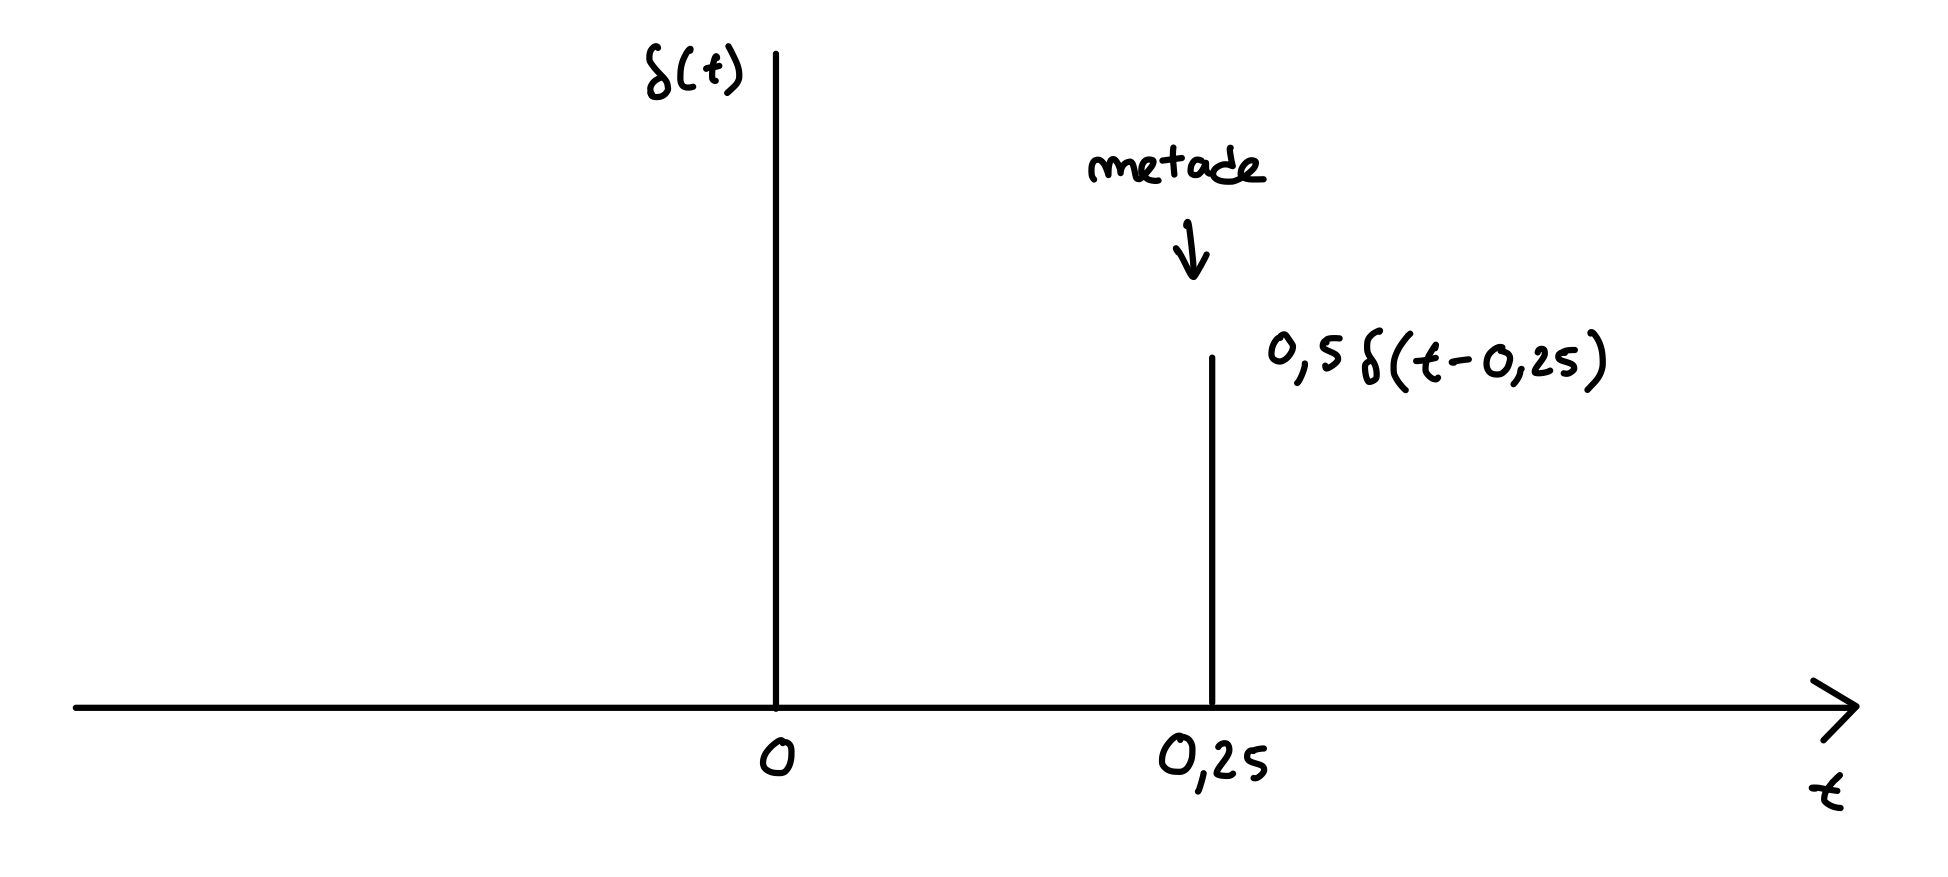
\includegraphics[width=12cm]{images/Graf3.png}
          \end{figure}
    \item \textbf{Q9:} O sistema apresentado $(y(t))$ possui memória visto que não depende apenas do valor de $x(t)$ mas sim de $x(t)$ e de $(t - 0.25)$. Para além disso é um sistema causal uma vez que o seu output depende apenas dos valores do presente $x(t)$ e do passado $x(t - 0.25)$. Em relação à sua estabilidade, pode-se afirmar que é um sistema estável, visto que não é possível encontrar nenhum input limitado que provocasse um output não limitado:\\
          Sendo $a, b$ números arbitrários que verificam as condições
          \[\begin{cases}
                  |x(t)| < a \\
                  |x(t - 0.25)| < b
              \end{cases}\]
          Então: $-a - 0.5b < y(t) < at + 0.5b$, o que representa um output limitado.
    \item \textbf{Q10:} O efeito produzido pelo sistema é um eco (prolongamento do som).
    \item \textbf{Q11:} $x_2(t) = \cos(44t)$, que pode ser escrito como
          \[x_2(t) = \frac{1}{2}e^{j44t} + \frac{1}{2}e^{-j44t}\]
          $y_2(t) = x_2(t) + 0.5x_2(t - 0.25) =$
          \[= \frac{1}{2}e^{j44t} + \frac{1}{2}e^{-j44t} + \frac{1}{2}\left(\frac{1}{2}e^{j44t - 0.25}+\frac{1}{2}e^{-j44t + 0.25}\right)\]
          \[= \frac{1}{2}e^{j44t} + \frac{1}{2}e^{-j44t} + \frac{1}{4}e^{j44t - 11} + \frac{1}{4}e^{-j44t + 11}\]
          \[= \frac{1}{2}e^{j44t} + \frac{1}{2}e^{-j44t} + \frac{1}{4e^{11}}e^{j44t} + \frac{e^{11}}{4}e^{-j44t}\]
          \[= \frac{2e^{11} + 1}{4e^{11}}e^{j44t} + \frac{2+e^{11}}{4}e^{-j44t}\]

\end{itemize}
\newpage
% % % % % % % % % % % % % % % % % % % % % % % % % % %
\section{Série de Fourier}
\newpage
% % % % % % % % % % % % % % % % % % % % % % % % % % %
\section{Resposta em Frequência}
\newpage
% % % % % % % % % % % % % % % % % % % % % % % % % % %
\section{Filtragem}
\begin{itemize}
    \item \textbf{Q23:} Sendo que um filtro passa-baixo apenas deixa passar as\\
          frequências baixas e rejeita as frequências mais altas, logo este não reproduz bem as zonas de variação rápida do sinal $p$, mas reproduz bem as zonas de variação lenta.\\
          Por sua vez o filtro passa-alto, como é o inverso do filtro passa-baixo, reproduz bem as zonas de variação rápida do sinal $p$, mas não reproduz bem as zonas de variação lenta.
\end{itemize}
\newpage
% % % % % % % % % % % % % % % % % % % % % % % % % % %
\section{Amostragem}
% % % % % % % % % % % % % % % % % % % % % % % % % % %
\end{document}